
\documentclass[article]{jss}
\usepackage[utf8]{inputenc}

\usepackage{amsmath, amsfonts, amssymb, amsthm, graphicx}
\usepackage[ruled]{algorithm2e}
\usepackage{caption}
\usepackage{tikz}

\setlength{\parindent}{0pt}
\newcommand{\forceindent}{\leavevmode{\parindent=1em\indent}}
\numberwithin{equation}{section}

\newtheorem*{theorem*}{Theorem}
\newtheorem*{cor*}{Corollary}

\newcommand{\norm}[1]{\left\lVert#1\right\rVert}
\newcommand{\e}{\epsilon}
\newcommand{\w}{\omega}
\newcommand{\R}{\mathbb{R}}
\newcommand{\N}{\mathbb{N}}
\newcommand{\Q}{\mathbb{Q}}
\newcommand{\Z}{\mathbb{Z}}
\renewcommand{\ae}[1]{\text{ \hspace{5pt} a.e. #1}}


\author{Austin David Brown\\University of Minnesota}

\title{Combining $l^1$ and Higher Order $l^p$ Penalization in Regression Models}

\Abstract{
We create the package Penalized Regression on Steroids (\textbf{pros}) to combine $l^1$ penalized regression with higher order $l^p$ penalizations built upon the Elasticnet idea. The package is able to fit regression models with penalizations ranging from $l^1$ to $l^{10}$.
}

\Keywords{Penalized Regression, \proglang{C++}, \proglang{Python}, \proglang{R}}
\Plainkeywords{Penalized Regression, C++, R, Python}

\Address{
  Austin David Brown \\
  University of Minnesota \\
  Department of Statistics (Graduate Student) \\
  E-mail: \email{Brow5079@umn.edu}
}

\begin{document}

\section{Introduction}

In statistics and probability theory it is common to impose moment assumptions on a random variable $X : \Omega \to \R^n$ such as $E(|X|^k) < \infty$ for $k \in \R$.
These constraints correspond to the $L^p$ spaces which allow control over the width and the height of such random variables.
We believe that analogous tools should be available for scientists tackling real problems.
The problem may also be motivated geometrically.
Consider for example an Elasticnet penalty $Q(x) = \frac{1}{2} |x| + \frac{1}{2} |y| + \frac{1}{2} |x|^2 + \frac{1}{2} |y|^2 \le 1$
shown on the left and a new penalty $P(x) = \frac{1}{2} |x| + \frac{1}{2} |y| + \frac{1}{2} |x|^4 + \frac{1}{2} |y|^4 \le 1$ shown on the right.


\begin{minipage}{.5\textwidth}
  \centering
  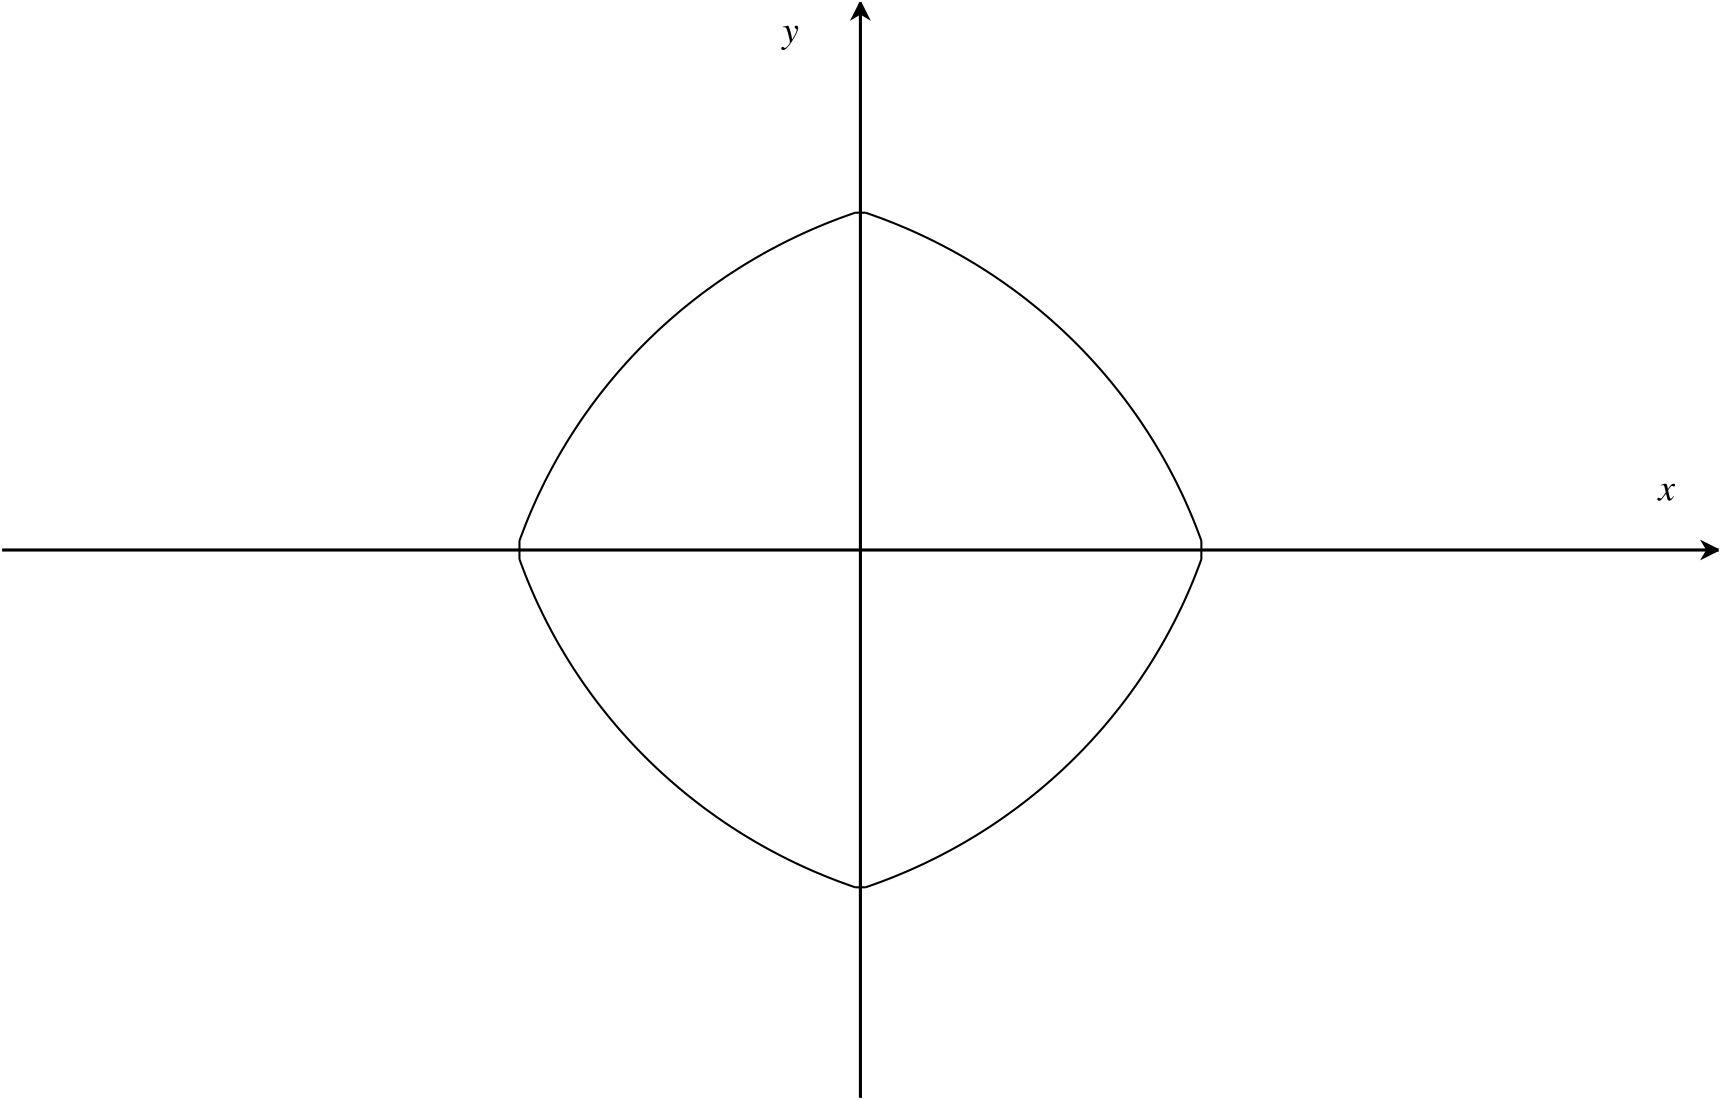
\includegraphics[width=.9\linewidth]{elasticnet.png}
\end{minipage}%
\begin{minipage}{.5\textwidth}
  \centering
  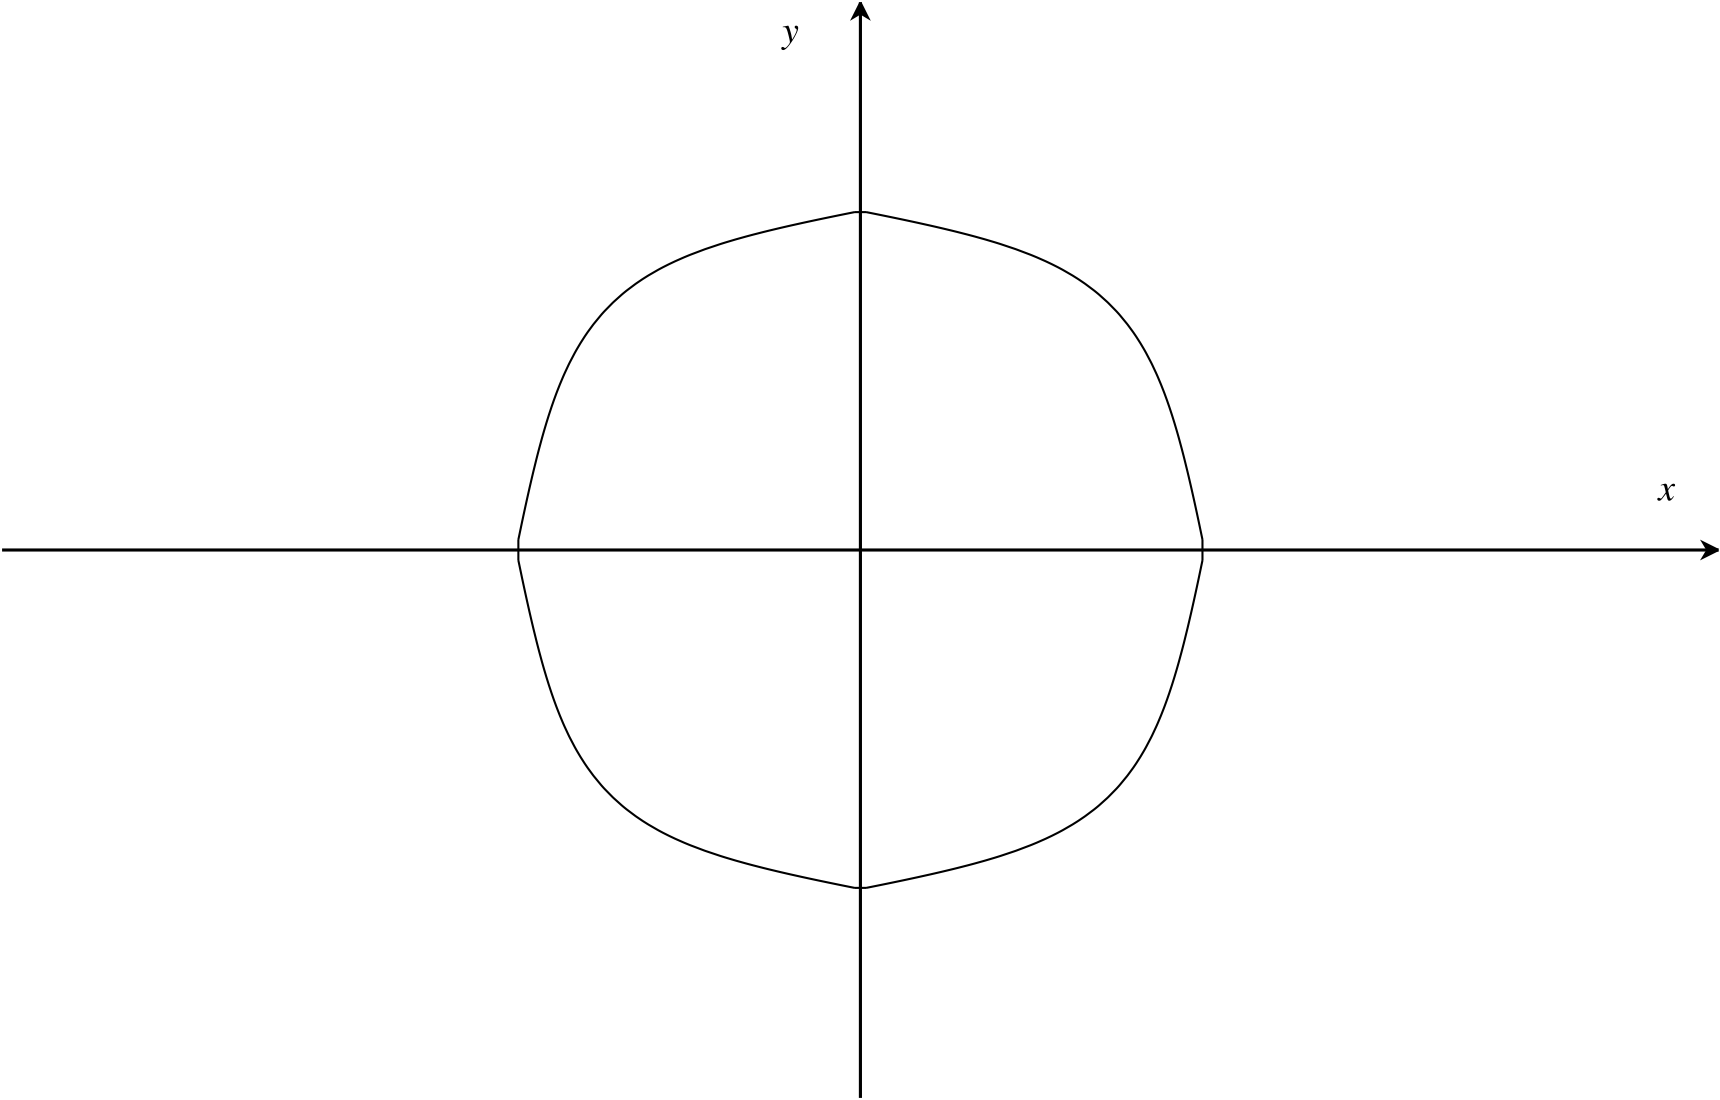
\includegraphics[width=.9\linewidth]{new_penalty_4_moment.png}
\end{minipage}
\captionof{figure}{A particular ElasticNet penalty shown on the left and a new penalty shown on the right shown to "bow" out the penalization while retaining convexity.}


A scientist may want the ability to control the height and width of the penalization while still retaining sparse solutions.
In this project, we build the Penalized Regression on Steroids (\textbf{pros}) package available to the R programming language to expand upon the idea of ElasticNet by \cite{elasticnet}, which we believe approximately encapsulates this idea.

\section{Penalized Regression Implementation}

In this section, we discuss how the package was implemented. In particular, the construction of the problem and the algorithms used.
Let
\[
L_{\lambda}(\beta) = \frac{1}{2} \norm{y - X \beta}_2^2 + \lambda P(\beta)
\]
be the objective to minimize with penalty
\[
\lambda P(\beta) = \lambda \alpha_0 \norm{\beta}_1 + \lambda \sum_{k = 1}^{5} \alpha_k \norm{\beta}_{2k}^{2k} 
\]
where $y \in \R^n$, $X \in M_{n \times p}(\R)$, and $\beta \in \R^p$, $\lambda \in \R_{+}$ and $\alpha$'s are convex combinations.
An important property of this penalty is convex and completely separable which allows for coordinate-wise optimization.
In \textbf{glmnet} by \cite{glmnet}, the authors use coordinate descent.
Further, with the Elasticnet penalty by \cite{elasticnet}, the coordinate wise minimization yields an analytic, closed form solution at each iteration avoiding any need for a line search or step size.
The penalty that we propose lacks an analytic solution and thus a new algorithm is needed.

\subsection{Optimization Algorithms and Implementation}

The first algorithm utilized was the subgradient coordinate algorithm shown below.

\vspace{.2cm}
\begin{algorithm}[H]
\caption{Subgradient Coordinate Algorithm}
Choose $\beta^0 \in \R^p$, tolerance $\delta > 0$, $R > 0$, and maximum iterations $N$.

Set $k \gets 0$

Set the step size $h \gets \frac{R}{\sqrt{1 + N}}$

\Repeat{Until the objective difference is less than $\delta$}{ 

  Permute $I = \{1, \ldots, p\}$

  \For {$i \in I$}{

    $\beta^{k + 1}_i \gets \beta^{k}_i - h g^i$ where $g^k_i \in (\partial L_\lambda(\beta^k))_i$

    $k \gets k + 1$
  }
}

\end{algorithm}
\vspace{.2cm}

The drawbacks of this algorithm include lack of the descent property, no good stopping criterion, and many possible choices for the subgradient.
The step size is optimal and chosen due to \cite{nesterov} with a worst case convergence rate of $O(\frac{1}{\sqrt{k}})$.
Ultimately, no line search can be implemented and the step size must be tuned by the user, which may be difficult for many users.
The stopping criterion is also expensive at $O(n^2)$ flops at each iteration.

Due to the separability of the penalization, a better algorithm is proximal gradient coordinate descent shown below.

\vspace{.2cm}
\begin{algorithm}[H]
\caption{Proximal Gradient Coordinate Descent}
Choose $\beta^0 \in \R^p$ and tolerance $\delta > 0$;

Set $k \gets 0$

\Repeat{Until the Moreau-Yoshida mapping $M_{h_k, f} < \delta$}{ 


  Randomly permute $I = \{1, \ldots, p\}$

  \For {$i \in I$}{
    Set the step size $h_i > 0$ or use line search.

    $\beta^{k + 1}_i \gets (\textbf{prox}_{h_i L})_i ( \beta^k_i - h^k \langle X_i, y - X \beta \rangle )$

    $k \gets k + 1$
  }

}
\end{algorithm}
\vspace{.2cm}

The major benefit of this algorithm is that it is a descent method and thus line search may be implemented.
Moreover, the stopping criterion is cheap to compute at $O(p)$ flops.
The Moreau-Yoshida map recovers the worst case convergence of $O(\frac{1}{k})$ generally and coordinate descent algorithms are explored by \cite{nesterov2}.

\subsection{Cross-Validation Algorithms and Implementation}

In order to tune the Lagrangian dual variable $\lambda$, K-fold cross validation is implemented.
To improve the speed of cross-validation, a warm start algorithm is used defined below.

\vspace{.2cm}
\begin{algorithm}[H]
\caption{Warm Start Cross-Validation}
Choose a sequence of Langrangian dual variables $\lambda_1, \ldots, \lambda_N$, and initial value $\beta^0$.

Order $\lambda_{(1)}, \ldots, \lambda_{(N)}$ descending.

$\beta^{Warm} \gets \beta^0$ 

\For{$k \in 1, \ldots, N$}{

  $\beta^k \gets$ by Cross-Validation with $\lambda_{(k)}$ warm started with $\beta^{Warm}$.

  $\beta^{Warm} \gets \beta^k$
}

\end{algorithm}
\vspace{.2cm}

A difficult problem in general is choosing the sequence of $\lambda$'s.
In \textbf{glmnet}, the default is to choose a sequence of length $100$ starting from the first $\lambda_{max}$ where $\beta$ is completely zero to the lower value $.001 \lambda_{max}$ on a log-scale.
We believe, the lower $\lambda$ value in the sequence is the real difficulty and this implementation does not address this.
Due to time, we implement a similar default choice.
We choose the lower $\lambda = c p$ where $c > 0$ is a tuning parameter and then create a sequence of length $100$ from this lower value.
The default choice comparisons are explored in a subsequent section.


\subsection{Discussion}

One source of serious confusion for the author that soaked up a lot of time was that \textbf{glmnet} uses a transformation for their $\lambda$ values and these do not correspond with the typical Lasso model. Thus, direct comparisons are extremely confusing.


\section{The Penalized Regression on Steroids Package}

\subsection{Package Architecture}

The package \textbf{pros} is built using C++ and the Eigen library by \cite{eigen} is utilized for fast matrix computations. This is analogous to using Fortran with LAPACK by \cite{lapack}.
The \textbf{pros} library is not dependent on R.
To interact with R, 2 interfacing layers are needed: an R to C interface and an R program defining user callable functions.
The benefit is that many other popular programming languages can be interfaced easily.
The following diagram illustrates this idea showing that the \textbf{pros} package is more general than just an R package.

\vspace{.5cm}
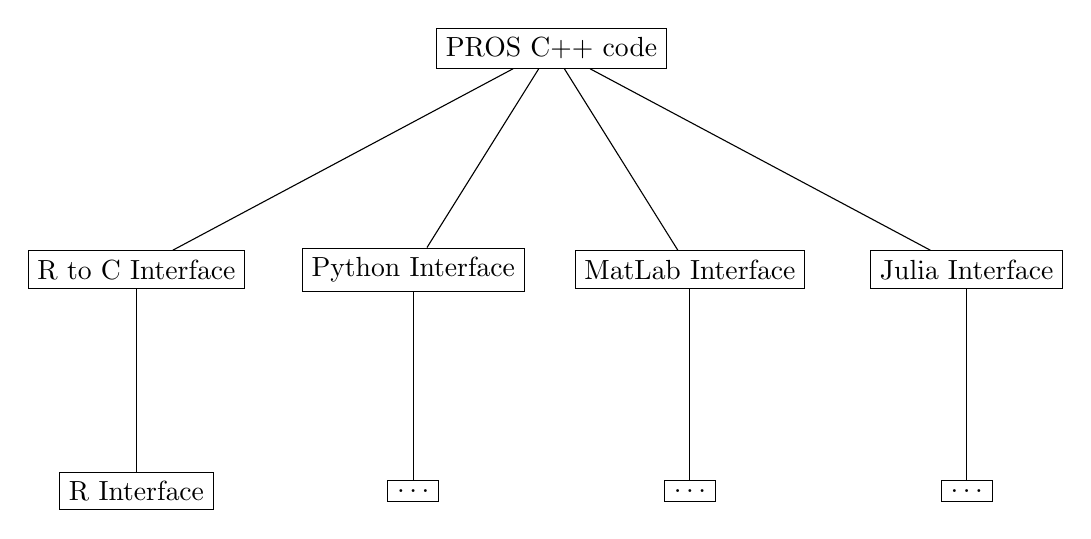
\begin{tikzpicture}[level distance=8em, sibling distance=10em,
  every node/.style = {shape=rectangle, draw, align=center}]]
  \node {PROS C++ code}
    child { node {R to C Interface} 
      child { node {R Interface} }
    }
    child { node {Python Interface} 
      child { node {$\ldots$} }
    }
    child { node {MatLab Interface} 
      child { node {$\ldots$} }
    }
    child { node {Julia Interface} 
      child { node {$\ldots$} }
    };
\end{tikzpicture}
\captionof{figure}{Illustrates interfacing the \textbf{pros} package with other languages.}
\vspace{.5cm}


The R interface in its simplest form is comprised of 2 functions.
A single fitting function with prediction

\begin{verbatim}
> fit <- pros(X, y, alpha)
> predict(fit, X)
\end{verbatim}

and a cross-validation function with prediction

\begin{verbatim}
> cv <- cv.pros(X, y, alpha)
> predict(cv, X)
\end{verbatim}

We illustrate the usage of these functions in the following sections.

\subsection{The Regression Fitting Function}

The \textbf{pros} function is used to fit a single regression model with a specified penalization. The signature of this function at the time of this paper is as follows:

\begin{itemize}
\item \code{X} is an $n \times m$-dimensional matrix of the data.

\item \code{y} is an $n$-dimensional vector of response values.

\item \code{alpha} is a $6$-dimensional vector of the convex combination corresponding to the penalization:
 \begin{itemize}
   \item $\alpha_1$ is the $l^1$ penalty.
   \item $\alpha_2$ is the $l^2$ penalty.
   \item $\alpha_3$ is the $l^4$ penalty.
   \item $\alpha_4$ is the $l^6$ penalty.
   \item $\alpha_5$ is the $l^8$ penalty.
   \item $\alpha_6$ is the $l^{10}$ penalty.
\end{itemize}

\item \code{lambdas} is a vector of dual penalization values to be evaluated.

\item \code{step\_size} is a tuning parameter defining the step size. Larger values are more aggressive and smaller values are less aggressive.

\item \code{algorithm} is the optimization algorithm
\begin{itemize}
\item \code{proximal_gradient_cd} uses proximal gradient coordinate descent.
\item \code{subgradient_cd} uses subgradient coordinate descent.
\end{itemize}

\item \code{max\_iter} is the maximum iterations the algorithm will run regardless of convergence.

\item \code{tolerance} is the accuracy of the stopping criterion.

\item \code{random seed} is the random seed used in the algorithms.

\end{itemize}

\subsection{The Cross-Validation Function}

The \textbf{cv.pros} function is used for cross-validation.
The signature of this function at the time of this paper is as follows:

\begin{itemize}
\item \code{X} is an $n \times m$-dimensional matrix of the data.

\item \code{y} is an $n$-dimensional vector of response values.

\item \code{alpha} is a $6$-dimensional vector of the convex combination corresponding to the penalization:
 \begin{itemize}
   \item $\alpha_1$ is the $l^1$ penalty.
   \item $\alpha_2$ is the $l^2$ penalty.
   \item $\alpha_3$ is the $l^4$ penalty.
   \item $\alpha_4$ is the $l^6$ penalty.
   \item $\alpha_5$ is the $l^8$ penalty.
   \item $\alpha_6$ is the $l^{10}$ penalty.
\end{itemize}

\item \code{lambda} is the Lagrangian dual penalization parameter.

\item \code{step\_size} is a tuning parameter defining the step size. Larger values are more aggressive and smaller values are less aggressive.

\item \code{algorithm} is the optimization algorithm
\begin{itemize}
\item \code{proximal_gradient_cd} uses proximal gradient coordinate descent.
\item \code{subgradient_cd} uses subgradient coordinate descent.
\end{itemize}

\item \code{max\_iter} is the maximum iterations the algorithm will run regardless of convergence.

\item \code{tolerance} is the accuracy of the stopping criterion.

\item \code{random seed} is the random seed used in the algorithms.

\end{itemize}

\section{Numerical Examples}

\subsection{The Boston Housing Dataset}

The Boston Housing dataset is popular from \cite{boston_housing}.
There are 13 predictors and the response is the median value of owner-occupied homes in \$1000's. The analysis is setup in the following way:

\begin{itemize}
\item The data is randomly split into a training set with 404 observations and a test set with 102 observations.


\item The predictor data is standardized.

\item The \textbf{glmnet} library and the \textbf{pros} library were used for fitting.

\item 10-fold cross-validation was used to tune the Lagrangian dual variable $\lambda$.

\item The source code for this analysis is openly available at the \textbf{pros} repository available here \cite{pros}.

\end{itemize}

We compare default settings between the libraries

\begin{center}
\setlength{\tabcolsep}{20pt} % Default value: 6pt
\renewcommand{\arraystretch}{1} % Default value: 1
\begin{tabular}{lllp{7.4cm}}
\hline
Penalty & Tuning & Test Mean Squared Error \\ \hline
Lasso (glmnet) & $\alpha = 1$ & TODO \\
ElasticNet (glmnet) & $\alpha = 1/2$  & TODO   \\
Lasso (pros) & $\alpha = 1$ &  \\
ElasticNet (pros) & $\alpha = 1/2$ &  \\
4th Moment (pros) & $\alpha = 1/2$ &  \\ \hline
\end{tabular}
\end{center}

Next, we compare tuned results using pros

\begin{center}
\setlength{\tabcolsep}{20pt} % Default value: 6pt
\renewcommand{\arraystretch}{1} % Default value: 1
\begin{tabular}{lllp{7.4cm}}
\hline
Penalty & Tuning & Test Mean Squared Error \\ \hline
ElasticNet (pros) & $\alpha = .98$ & TODO \\
4th Moment (pros) & $\alpha = 0.96$ &  TODO \\
10th Moment (pros) & $\alpha = 0.96$ &  TODo \\ \hline
\end{tabular}
\end{center}

\subsection{The Prostate Dataset Analysis}

This is a popular dataset from \cite{prostate} and analyzed in the ElasticNet paper \cite{elasticnet}.
There are 8 predictors and the response is the log of the prostate specific antigen. The analysis is setup in the following way:

\begin{itemize}
\item The data is split into a training set with 67 observations and a test set with 30 observations.

\item The predictor data is standardized.

\item The \textbf{glmnet} library and the \textbf{pros} library were used for fitting.

\item 10-fold cross-validation was used to choose the Lagrangian dual variable $\lambda$.

\item The source code for this analysis is openly available at the \textbf{pros} repository available here \cite{pros}.

\end{itemize}


We compare default settings between the libraries

\begin{center}
\setlength{\tabcolsep}{20pt} % Default value: 6pt
\renewcommand{\arraystretch}{1} % Default value: 1
\begin{tabular}{lllp{7.4cm}}
\hline
Penalty & Tuning & Test Mean Squared Error \\ \hline
Lasso (glmnet) & $\alpha = 1$ & 0.4443432-0.4646501 \\
ElasticNet (glmnet) & $\alpha = 1/2$  & 0.4539684-0.4554527   \\
Lasso (pros) & $\alpha = 1$ &  \\
ElasticNet (pros) & $\alpha = 1/2$ &  \\
4th Moment (pros) & $\alpha = 1/2$ &  \\ \hline
\end{tabular}
\end{center}

Next, we compare tuned results using pros

\begin{center}
\setlength{\tabcolsep}{20pt} % Default value: 6pt
\renewcommand{\arraystretch}{1} % Default value: 1
\begin{tabular}{lllp{7.4cm}}
\hline
Penalty & Tuning & Test Mean Squared Error \\ \hline
ElasticNet (pros) & $\alpha = .98$ & 0.4442702 \\
4th Moment (pros) & $\alpha = 0.96$ &  0.4441759 \\
10th Moment (pros) & $\alpha = 0.96$ &  0.4441322 \\ \hline
\end{tabular}
\end{center}


\bibliography{project}

\end{document}

